\documentclass[12pt, a4paper]{article}
\usepackage[letterpaper, hmargin=0.75in, vmargin=0.75in]{geometry}
\usepackage{graphicx}
\usepackage[hyphens]{url}
\usepackage{hyperref}
\usepackage{listings}
\usepackage{pgf}
\usepackage{tikz}
\usepackage{courier}
\usepackage{amsfonts,amssymb,amsmath,amsthm,lastpage,fancyhdr,wrapfig,multirow}
\usepackage{palatino}
\usepackage{amsmath}
\usepackage[english]{babel}
\usepackage[utf8]{inputenc}
\usepackage{fancyhdr}
\textwidth 7.5in
\oddsidemargin -.5in
\topmargin -0.70in
\textheight 9.8in                      

\pagestyle{fancy}

%**************Fill in your ID and initials here*****************
\newcommand{\mc}[1]{\ensuremath{\mathcal{{#1}}}}
\newcommand{\mb}[1]{\ensuremath{\mathbb{{#1}}}}
\newcommand{\mf}[1]{\ensuremath{\mathfrak{{#1}}}}
\newcommand{\N}[1]{\ensuremath{\{1,\ldots,{#1}\}}}

\newcommand{\Worth}[1]{\{{#1} marks\}}
\newcommand{\Sln}{\smallskip \textbf{Solution.} }
\newcommand{\Extra}[1]{\{Extra credit: {#1} marks\}}


\setlength{\parskip}{0.15in}
\setlength{\parindent}{0in}


\newcommand{\NP}{\newpage \vspace*{-0.4in}}
\newcommand{\FP}{\vspace*{-0.6in}}
\newcommand{\tab}[1][1cm]{\hspace*{#1}}
\newcommand{\ES}{Erwin Schr\"odinger}

\lstset{ %
basicstyle=\ttfamily\scriptsize,commentstyle=\scriptsize\itshape,showstringspaces=false,breaklines=true}

\tikzstyle{input} = [coordinate]
\tikzstyle{output} = [coordinate]
\tikzstyle{joint} = [draw, circle, minimum size=1em]
\tikzstyle{block} = [draw, rectangle, minimum height=3em, minimum width=6em]


\title{\huge SE380 Notes}
\author{Minyang Jiang}
\date{\today}

\begin{document}

\maketitle

\NP
\section*{Introduction}
\subsection*{What is control engineering?}
Example (automated highway)
\begin{center}
  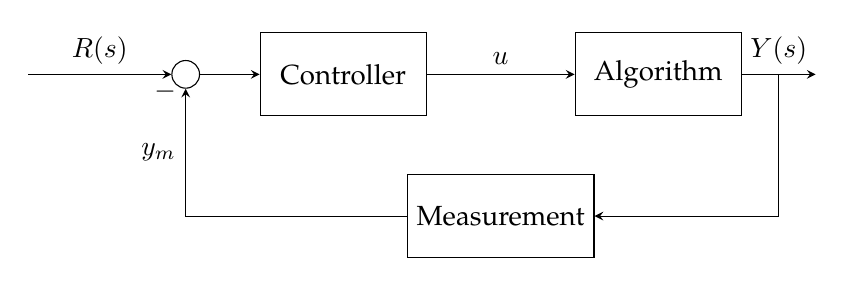
\begin{tikzpicture}[auto, node distance=2cm, >=stealth]
    \node [input, name=input] (input) {};
    \node [joint, right of=input] (joint1) {};
    \node [block, right of=joint1] (controller) {Controller};
    \node [block, right of=controller, node distance=4cm] (algorithm) {Algorithm};
    \draw [->] (controller) -- node[name=u] {$u$} (algorithm);
    \node [block, below of=u] (measurement) {Measurement};
    \node [output, right of=algorithm] (output) {};

    \draw [->] (input) -- node{$R(s)$} (joint1);
    \draw [->] (joint1) -- node{} (controller);
    \draw [->] (algorithm) -- node[name=y]{$Y(s)$} (output);
    \draw [->] (y) |- node{} (measurement);
    \draw [->] (measurement) -| node[pos=0.99]{$-$} node [near end]{$y_m$} (joint1);

  \end{tikzpicture}
\end{center}
\end{document}